%% bare_jrnl.tex
%% V1.4b
%% 2015/08/26
%% by Michael Shell
%% see http://www.michaelshell.org/
%% for current contact information.
%%
%% This is a skeleton file demonstrating the use of IEEEtran.cls
%% (requires IEEEtran.cls version 1.8b or later) with an IEEE
%% journal paper.
%%
%% Support sites:
%% http://www.michaelshell.org/tex/ieeetran/
%% http://www.ctan.org/pkg/ieeetran
%% and
%% http://www.ieee.org/

%%*************************************************************************
%% Legal Notice:
%% This code is offered as-is without any warranty either expressed or
%% implied; without even the implied warranty of MERCHANTABILITY or
%% FITNESS FOR A PARTICULAR PURPOSE!
%% User assumes all risk.
%% In no event shall the IEEE or any contributor to this code be liable for
%% any damages or losses, including, but not limited to, incidental,
%% consequential, or any other damages, resulting from the use or misuse
%% of any information contained here.
%%
%% All comments are the opinions of their respective authors and are not
%% necessarily endorsed by the IEEE.
%%
%% This work is distributed under the LaTeX Project Public License (LPPL)
%% ( http://www.latex-project.org/ ) version 1.3, and may be freely used,
%% distributed and modified. A copy of the LPPL, version 1.3, is included
%% in the base LaTeX documentation of all distributions of LaTeX released
%% 2003/12/01 or later.
%% Retain all contribution notices and credits.
%% ** Modified files should be clearly indicated as such, including  **
%% ** renaming them and changing author support contact information. **
%%*************************************************************************


% *** Authors should verify (and, if needed, correct) their LaTeX system  ***
% *** with the testflow diagnostic prior to trusting their LaTeX platform ***
% *** with production work. The IEEE's font choices and paper sizes can   ***
% *** trigger bugs that do not appear when using other class files.       ***                          ***
% The testflow support page is at:
% http://www.michaelshell.org/tex/testflow/



\documentclass[journal]{IEEEtran}
%
% If IEEEtran.cls has not been installed into the LaTeX system files,
% manually specify the path to it like:
% \documentclass[journal]{../sty/IEEEtran}



% Some very useful LaTeX packages include:
% (uncomment the ones you want to load)


% *** MISC UTILITY PACKAGES ***
%
%\usepackage{ifpdf}
% Heiko Oberdiek's ifpdf.sty is very useful if you need conditional
% compilation based on whether the output is pdf or dvi.
% usage:
% \ifpdf
%   % pdf code
% \else
%   % dvi code
% \fi
% The latest version of ifpdf.sty can be obtained from:
% http://www.ctan.org/pkg/ifpdf
% Also, note that IEEEtran.cls V1.7 and later provides a builtin
% \ifCLASSINFOpdf conditional that works the same way.
% When switching from latex to pdflatex and vice-versa, the compiler may
% have to be run twice to clear warning/error messages.





% *** CITATION PACKAGES ***
%
%\usepackage{cite}
% cite.sty was written by Donald Arseneau
% V1.6 and later of IEEEtran pre-defines the format of the cite.sty package
% \cite{} output to follow that of the IEEE. Loading the cite package will
% result in citation numbers being automatically sorted and properly
% "compressed/ranged". e.g., [1], [9], [2], [7], [5], [6] without using
% cite.sty will become [1], [2], [5]--[7], [9] using cite.sty. cite.sty's
% \cite will automatically add leading space, if needed. Use cite.sty's
% noadjust option (cite.sty V3.8 and later) if you want to turn this off
% such as if a citation ever needs to be enclosed in parenthesis.
% cite.sty is already installed on most LaTeX systems. Be sure and use
% version 5.0 (2009-03-20) and later if using hyperref.sty.
% The latest version can be obtained at:
% http://www.ctan.org/pkg/cite
% The documentation is contained in the cite.sty file itself.






% *** GRAPHICS RELATED PACKAGES ***
%
\ifCLASSINFOpdf
  \usepackage[pdftex]{graphicx}
  % declare the path(s) where your graphic files are
  % \graphicspath{{../pdf/}{../jpeg/}}
  % and their extensions so you won't have to specify these with
  % every instance of \includegraphics
  % \DeclareGraphicsExtensions{.pdf,.jpeg,.png}
\else
  % or other class option (dvipsone, dvipdf, if not using dvips). graphicx
  % will default to the driver specified in the system graphics.cfg if no
  % driver is specified.
  % \usepackage[dvips]{graphicx}
  % declare the path(s) where your graphic files are
  % \graphicspath{{../eps/}}
  % and their extensions so you won't have to specify these with
  % every instance of \includegraphics
  % \DeclareGraphicsExtensions{.eps}
\fi
% graphicx was written by David Carlisle and Sebastian Rahtz. It is
% required if you want graphics, photos, etc. graphicx.sty is already
% installed on most LaTeX systems. The latest version and documentation
% can be obtained at:
% http://www.ctan.org/pkg/graphicx
% Another good source of documentation is "Using Imported Graphics in
% LaTeX2e" by Keith Reckdahl which can be found at:
% http://www.ctan.org/pkg/epslatex
%
% latex, and pdflatex in dvi mode, support graphics in encapsulated
% postscript (.eps) format. pdflatex in pdf mode supports graphics
% in .pdf, .jpeg, .png and .mps (metapost) formats. Users should ensure
% that all non-photo figures use a vector format (.eps, .pdf, .mps) and
% not a bitmapped formats (.jpeg, .png). The IEEE frowns on bitmapped formats
% which can result in "jaggedy"/blurry rendering of lines and letters as
% well as large increases in file sizes.
%
% You can find documentation about the pdfTeX application at:
% http://www.tug.org/applications/pdftex


\usepackage[framemethod=TikZ]{mdframed}
\usepackage{booktabs}
\usepackage[table]{xcolor}

% ===========================================================================================
% TIKZ PACKAGES AND CONFIGURATION
% ===========================================================================================
\usepackage{tikz}
\usepackage{pgfplots}
\pgfplotsset{compat=1.9}

% TikZ Libraries
\usetikzlibrary{patterns}
\usetikzlibrary{positioning}
\usetikzlibrary{fit}
\usetikzlibrary{calc}

% ===========================================================================================
% COLOR DEFINITIONS FOR CHARTS
% ===========================================================================================
\definecolor{rosso}{RGB}{220,57,18}
\definecolor{giallo}{RGB}{255,153,0}
\definecolor{blu}{RGB}{102,140,217}
\definecolor{verde}{RGB}{16,150,24}
\definecolor{viola}{RGB}{153,0,153}
\definecolor{hardblue}{RGB}{51,102,204}

% ===========================================================================================
% TIKZ STYLES FOR PIE CHARTS
% ===========================================================================================
\tikzset{
  chart/.style={
    legend label/.style={font={\scriptsize},anchor=west,align=left},
    legend box/.style={rectangle, draw, minimum size=10pt},
    axis/.style={black,semithick,->},
    axis label/.style={anchor=east,font={\tiny}},
  },
  pie chart/.style={
    chart,
    slice/.style={line cap=round, line join=round, very thick,draw=white},
    pie title/.style={font={\bfseries}},
    slice type/.style n args={3}{
        ##1/.style={pattern color=##2,pattern=##3},
        values of ##1/.style={
            black,
            font=\footnotesize,
            text opacity=1,
            fill=white,
            fill opacity=0.5,
            outer sep=\pgflinewidth
        }
    }
  }
}

% Layers for pie charts
\pgfdeclarelayer{background}
\pgfdeclarelayer{foreground}
\pgfsetlayers{background,main,foreground}

% Pie chart command
\newcommand{\pie}[3][]{
    \begin{scope}[#1]
    \pgfmathsetmacro{\curA}{90}
    \pgfmathsetmacro{\r}{1}
    \def\c{(0,0)}
    \def\offset{0}
    \foreach \v/\s/\number in{#3}{
        \pgfmathsetmacro{\deltaA}{\v/100*360}
        \pgfmathsetmacro{\nextA}{\curA + \deltaA}
        \pgfmathsetmacro{\midA}{(\curA+\nextA)/2}

        \path[slice,\s] \c
            -- +(\curA:\r)
            arc (\curA:\nextA:\r)
            -- cycle;
        \pgfmathsetmacro{\d}{max((\deltaA * -(.5/50) + 1) , .5)}

        \begin{pgfonlayer}{foreground}
        \path \c -- node[pos=\d+\offset,pie values,values of \s]{\number\hspace{.8mm}($\v\%$)} +(\midA:\r);
        \end{pgfonlayer}

        \global\let\curA\nextA
    }
    \end{scope}
}

% Legend command
\newcommand{\legendchart}[2][]{
    \begin{scope}[#1]
    \path
        \foreach \n/\s in {#2}
        {
            ++(0,-4pt) node[\s,legend box] {} +(2pt,0) node[legend label] {\n}
        }
    ;
    \end{scope}
}



% *** MATH PACKAGES ***
%
%\usepackage{amsmath}
% A popular package from the American Mathematical Society that provides
% many useful and powerful commands for dealing with mathematics.
%
% Note that the amsmath package sets \interdisplaylinepenalty to 10000
% thus preventing page breaks from occurring within multiline equations. Use:
%\interdisplaylinepenalty=2500
% after loading amsmath to restore such page breaks as IEEEtran.cls normally
% does. amsmath.sty is already installed on most LaTeX systems. The latest
% version and documentation can be obtained at:
% http://www.ctan.org/pkg/amsmath





% *** SPECIALIZED LIST PACKAGES ***
%
%\usepackage{algorithmic}
% algorithmic.sty was written by Peter Williams and Rogerio Brito.
% This package provides an algorithmic environment fo describing algorithms.
% You can use the algorithmic environment in-text or within a figure
% environment to provide for a floating algorithm. Do NOT use the algorithm
% floating environment provided by algorithm.sty (by the same authors) or
% algorithm2e.sty (by Christophe Fiorio) as the IEEE does not use dedicated
% algorithm float types and packages that provide these will not provide
% correct IEEE style captions. The latest version and documentation of
% algorithmic.sty can be obtained at:
% http://www.ctan.org/pkg/algorithms
% Also of interest may be the (relatively newer and more customizable)
% algorithmicx.sty package by Szasz Janos:
% http://www.ctan.org/pkg/algorithmicx

\usepackage{enumitem}


% *** ALIGNMENT PACKAGES ***
%
%\usepackage{array}
% Frank Mittelbach's and David Carlisle's array.sty patches and improves
% the standard LaTeX2e array and tabular environments to provide better
% appearance and additional user controls. As the default LaTeX2e table
% generation code is lacking to the point of almost being broken with
% respect to the quality of the end results, all users are strongly
% advised to use an enhanced (at the very least that provided by array.sty)
% set of table tools. array.sty is already installed on most systems. The
% latest version and documentation can be obtained at:
% http://www.ctan.org/pkg/array


% IEEEtran contains the IEEEeqnarray family of commands that can be used to
% generate multiline equations as well as matrices, tables, etc., of high
% quality.




% *** SUBFIGURE PACKAGES ***
%\ifCLASSOPTIONcompsoc
%  \usepackage[caption=false,font=normalsize,labelfont=sf,textfont=sf]{subfig}
%\else
%  \usepackage[caption=false,font=footnotesize]{subfig}
%\fi
% subfig.sty, written by Steven Douglas Cochran, is the modern replacement
% for subfigure.sty, the latter of which is no longer maintained and is
% incompatible with some LaTeX packages including fixltx2e. However,
% subfig.sty requires and automatically loads Axel Sommerfeldt's caption.sty
% which will override IEEEtran.cls' handling of captions and this will result
% in non-IEEE style figure/table captions. To prevent this problem, be sure
% and invoke subfig.sty's "caption=false" package option (available since
% subfig.sty version 1.3, 2005/06/28) as this is will preserve IEEEtran.cls
% handling of captions.
% Note that the Computer Society format requires a larger sans serif font
% than the serif footnote size font used in traditional IEEE formatting
% and thus the need to invoke different subfig.sty package options depending
% on whether compsoc mode has been enabled.
%
% The latest version and documentation of subfig.sty can be obtained at:
% http://www.ctan.org/pkg/subfig




% *** FLOAT PACKAGES ***
%
%\usepackage{fixltx2e}
% fixltx2e, the successor to the earlier fix2col.sty, was written by
% Frank Mittelbach and David Carlisle. This package corrects a few problems
% in the LaTeX2e kernel, the most notable of which is that in current
% LaTeX2e releases, the ordering of single and double column floats is not
% guaranteed to be preserved. Thus, an unpatched LaTeX2e can allow a
% single column figure to be placed prior to an earlier double column
% figure.
% Be aware that LaTeX2e kernels dated 2015 and later have fixltx2e.sty's
% corrections already built into the system in which case a warning will
% be issued if an attempt is made to load fixltx2e.sty as it is no longer
% needed.
% The latest version and documentation can be found at:
% http://www.ctan.org/pkg/fixltx2e


%\usepackage{stfloats}
% stfloats.sty was written by Sigitas Tolusis. This package gives LaTeX2e
% the ability to do double column floats at the bottom of the page as well
% as the top. (e.g., "\begin{figure*}[!b]" is not normally possible in
% LaTeX2e). It also provides a command:
%\fnbelowfloat
% to enable the placement of footnotes below bottom floats (the standard
% LaTeX2e kernel puts them above bottom floats). This is an invasive package
% which rewrites many portions of the LaTeX2e float routines. It may not work
% with other packages that modify the LaTeX2e float routines. The latest
% version and documentation can be obtained at:
% http://www.ctan.org/pkg/stfloats
% Do not use the stfloats baselinefloat ability as the IEEE does not allow
% \baselineskip to stretch. Authors submitting work to the IEEE should note
% that the IEEE rarely uses double column equations and that authors should try
% to avoid such use. Do not be tempted to use the cuted.sty or midfloat.sty
% packages (also by Sigitas Tolusis) as the IEEE does not format its papers in
% such ways.
% Do not attempt to use stfloats with fixltx2e as they are incompatible.
% Instead, use Morten Hogholm'a dblfloatfix which combines the features
% of both fixltx2e and stfloats:
%
% \usepackage{dblfloatfix}
% The latest version can be found at:
% http://www.ctan.org/pkg/dblfloatfix




%\ifCLASSOPTIONcaptionsoff
%  \usepackage[nomarkers]{endfloat}
% \let\MYoriglatexcaption\caption
% \renewcommand{\caption}[2][\relax]{\MYoriglatexcaption[#2]{#2}}
%\fi
% endfloat.sty was written by James Darrell McCauley, Jeff Goldberg and
% Axel Sommerfeldt. This package may be useful when used in conjunction with
% IEEEtran.cls'  captionsoff option. Some IEEE journals/societies require that
% submissions have lists of figures/tables at the end of the paper and that
% figures/tables without any captions are placed on a page by themselves at
% the end of the document. If needed, the draftcls IEEEtran class option or
% \CLASSINPUTbaselinestretch interface can be used to increase the line
% spacing as well. Be sure and use the nomarkers option of endfloat to
% prevent endfloat from "marking" where the figures would have been placed
% in the text. The two hack lines of code above are a slight modification of
% that suggested by in the endfloat docs (section 8.4.1) to ensure that
% the full captions always appear in the list of figures/tables - even if
% the user used the short optional argument of \caption[]{}.
% IEEE papers do not typically make use of \caption[]'s optional argument,
% so this should not be an issue. A similar trick can be used to disable
% captions of packages such as subfig.sty that lack options to turn off
% the subcaptions:
% For subfig.sty:
% \let\MYorigsubfloat\subfloat
% \renewcommand{\subfloat}[2][\relax]{\MYorigsubfloat[]{#2}}
% However, the above trick will not work if both optional arguments of
% the \subfloat command are used. Furthermore, there needs to be a
% description of each subfigure *somewhere* and endfloat does not add
% subfigure captions to its list of figures. Thus, the best approach is to
% avoid the use of subfigure captions (many IEEE journals avoid them anyway)
% and instead reference/explain all the subfigures within the main caption.
% The latest version of endfloat.sty and its documentation can obtained at:
% http://www.ctan.org/pkg/endfloat
%
% The IEEEtran \ifCLASSOPTIONcaptionsoff conditional can also be used
% later in the document, say, to conditionally put the References on a
% page by themselves.




% *** PDF, URL AND HYPERLINK PACKAGES ***
%
\usepackage{url}
% url.sty was written by Donald Arseneau. It provides better support for
% handling and breaking URLs. url.sty is already installed on most LaTeX
% systems. The latest version and documentation can be obtained at:
% http://www.ctan.org/pkg/url
% Basically, \url{my_url_here}.




% *** Do not adjust lengths that control margins, column widths, etc. ***
% *** Do not use packages that alter fonts (such as pslatex).         ***
% There should be no need to do such things with IEEEtran.cls V1.6 and later.
% (Unless specifically asked to do so by the journal or conference you plan
% to submit to, of course. )


% correct bad hyphenation here
\hyphenation{op-tical net-works semi-conduc-tor}


\begin{document}
%
% paper title
% Titles are generally capitalized except for words such as a, an, and, as,
% at, but, by, for, in, nor, of, on, or, the, to and up, which are usually
% not capitalized unless they are the first or last word of the title.
% Linebreaks \\ can be used within to get better formatting as desired.
% Do not put math or special symbols in the title.
\title{Bare Demo of IEEEtran.cls\\ for IEEE Journals}
%
%
% author names and IEEE memberships
% note positions of commas and nonbreaking spaces ( ~ ) LaTeX will not break
% a structure at a ~ so this keeps an author's name from being broken across
% two lines.
% use \thanks{} to gain access to the first footnote area
% a separate \thanks must be used for each paragraph as LaTeX2e's \thanks
% was not built to handle multiple paragraphs
%

\author{Rafael~Ribeiro,~\IEEEmembership{Mestrando,~UNIPAMPA,}
        John~Doe,~\IEEEmembership{Fellow,~OSA,}
        and~Jane~Doe,~\IEEEmembership{Life~Fellow,~IEEE}% <-this % stops a space
\thanks{M. Shell was with the Department
of Electrical and Computer Engineering, Georgia Institute of Technology, Atlanta,
GA, 30332 USA e-mail: (see http://www.michaelshell.org/contact.html).}% <-this % stops a space
\thanks{J. Doe and J. Doe are with Anonymous University.}% <-this % stops a space
\thanks{Manuscript received April 19, 2005; revised August 26, 2015.}}

% note the % following the last \IEEEmembership and also \thanks -
% these prevent an unwanted space from occurring between the last author name
% and the end of the author line. i.e., if you had this:
%
% \author{....lastname \thanks{...} \thanks{...} }
%                     ^------------^------------^----Do not want these spaces!
%
% a space would be appended to the last name and could cause every name on that
% line to be shifted left slightly. This is one of those "LaTeX things". For
% instance, "\textbf{A} \textbf{B}" will typeset as "A B" not "AB". To get
% "AB" then you have to do: "\textbf{A}\textbf{B}"
% \thanks is no different in this regard, so shield the last } of each \thanks
% that ends a line with a % and do not let a space in before the next \thanks.
% Spaces after \IEEEmembership other than the last one are OK (and needed) as
% you are supposed to have spaces between the names. For what it is worth,
% this is a minor point as most people would not even notice if the said evil
% space somehow managed to creep in.



% The paper headers
\markboth{Journal of \LaTeX\ Class Files,~Vol.~14, No.~8, August~2015}%
{Shell \MakeLowercase{\textit{et al.}}: Bare Demo of IEEEtran.cls for IEEE Journals}
% The only time the second header will appear is for the odd numbered pages
% after the title page when using the twoside option.
%
% *** Note that you probably will NOT want to include the author's ***
% *** name in the headers of peer review papers.                   ***
% You can use \ifCLASSOPTIONpeerreview for conditional compilation here if
% you desire.




% If you want to put a publisher's ID mark on the page you can do it like
% this:
%\IEEEpubid{0000--0000/00\$00.00~\copyright~2015 IEEE}
% Remember, if you use this you must call \IEEEpubidadjcol in the second
% column for its text to clear the IEEEpubid mark.



% use for special paper notices
%\IEEEspecialpapernotice{(Invited Paper)}




% make the title area
\maketitle

% As a general rule, do not put math, special symbols or citations
% in the abstract or keywords.
\begin{abstract}
    \textbf{Context}: In the software lifecycle, the market introduction phase presents significant challenges related to business model definition and selection. This raises questions such as which business models are available, which are most commonly adopted, which best fit the proposed solution, what benefits and limitations they present, and how to choose the most appropriate model.
    \textbf{Objective}: This study aims to map and categorize software business models, providing a structured view that supports understanding, comparison, and strategic selection.
    \textbf{Method}: A Systematic Literature Review (SLR) was conducted using primary studies from the last decade (2014--2024) indexed in the ACM, IEEE Xplore, and Scopus digital libraries. Data extraction employed 33 extraction questions (12 closed-ended and 21 open-ended), with qualitative analysis using a coding scheme of 61 codes organized in 9 classes.
    \textbf{Results}: The search retrieved 2,889 studies, with 216 removed as duplicates. After title and abstract screening, 312 studies were considered potentially relevant, and the full-text quality assessment resulted in 67 studies included in the final synthesis. The analysis identified platform-based models (391 mentions), SaaS (289), freemium (264), and open source (188) as the most prevalent. Subscription-based revenue dominated at 76.1\%, with multi-tenant SaaS present in 71.6\% of studies. Key success factors include ecosystem management (138 mentions) and market expansion (84), while main challenges involve security concerns (41) and revenue stream transformation (38).
    \textbf{Conclusion}: The consolidated results provide a three-dimensional taxonomy (delivery, monetization, ecosystem) and serve as conceptual foundation for developing an ontology to represent software business models, contributing to the systematization of knowledge and supporting evidence-based strategic decision-making.
\end{abstract}

% Note that keywords are not normally used for peerreview papers.
\begin{IEEEkeywords}
Business Model, Software, Systematic Literature Review.
\end{IEEEkeywords}






% For peer review papers, you can put extra information on the cover
% page as needed:
% \ifCLASSOPTIONpeerreview
% \begin{center} \bfseries EDICS Category: 3-BBND \end{center}
% \fi
%
% For peerreview papers, this IEEEtran command inserts a page break and
% creates the second title. It will be ignored for other modes.
\IEEEpeerreviewmaketitle



\section{Introdução}\label{sec:intro}
% The very first letter is a 2 line initial drop letter followed
% by the rest of the first word in caps.
%
% form to use if the first word consists of a single letter:
% \IEEEPARstart{A}{demo} file is ....
%
% form to use if you need the single drop letter followed by
% normal text (unknown if ever used by the IEEE):
% \IEEEPARstart{A}{}demo file is ....
%
% Some journals put the first two words in caps:
% \IEEEPARstart{T}{his demo} file is ....
%
% Here we have the typical use of a "T" for an initial drop letter
% and "HIS" in caps to complete the first word.
\IEEEPARstart{O}{} desenvolvimento de software é um processo dinâmico que vai além da criação de código ou da entrega de funcionalidades. No ciclo de vida do software, a fase de inserção no mercado se apresenta como um momento crucial, no qual as decisões relacionadas à monetização e à sustentabilidade financeira precisam ser cuidadosamente planejadas. Nesse contexto, a modelagem de negócios desempenha um papel central, oferecendo estruturas para alinhar os objetivos estratégicos da organização com as necessidades do mercado.
% You must have at least 2 lines in the paragraph with the drop letter
% (should never be an issue)

Diferentes modelos de negócios, como o licenciamento, o modelo \textit{freemium} ou o software como serviço (SaaS), têm sido amplamente explorados na indústria de software. Entretanto, a escolha do modelo mais adequado para um produto específico envolve a consideração de diversos fatores, como tendências de mercado, desafios de implementação e práticas eficazes para mitigar riscos. Além disso, a literatura sobre modelos de negócios frequentemente aborda aspectos variados, dificultando a identificação de abordagens emergentes e bem-sucedidas no setor.

Dada essa complexidade, este estudo tem como objetivo explorar os modelos de negócios aplicados à indústria de software por meio de uma revisão sistemática da literatura (RSL) dos últimos 10 anos (2014–2024). A pesquisa busca responder a perguntas fundamentais sobre quais modelos têm sido utilizados, quais fatores influenciam sua escolha e quais práticas foram eficazes na superação de desafios de implementação. Para tanto, foram definidos critérios rigorosos para seleção, avaliação e extração de dados, garantindo a qualidade e a relevância dos estudos analisados.

Os resultados deste trabalho visam contribuir para a criação de uma ontologia que apoie tanto pesquisadores quanto profissionais na escolha e implementação de modelos de negócios eficazes para produtos de software. Ao compreender as características, fatores de sucesso e desafios de cada abordagem, este estudo fornece \textit{insights} valiosos para decisões estratégicas na indústria de software.

The remainder of this article is organized as follows: Section~\ref{sec:methodology} presents the methodology used, including the research questions, selection criteria, and extraction strategy; Section~\ref{sec:analysis} presents the analysis of results organized by research question; Section~\ref{sec:discussion} discusses the main findings and their implications; Section~\ref{sec:threats} addresses threats to validity; and Section~\ref{sec:conclusion} presents conclusions and future work.






\section{Fundamentação Teórica}





\section{Trabalhos Relacionados}





\section{Metodologia}\label{sec:methodology} %Protocolo e as etapas da execução
    \IEEEPARstart{E}{xistem} diversas diretrizes propostas para a realização de Revisão Sistemática da Literatura (RSL) e Mapeamento Sistemático da Literatura (MSL), como as apresentadas por \cite{keele2007guidelines}, \cite{engstrom2011software} e \cite{petersen2008systematic}.
    Este estudo seguiu principalmente as diretrizes descritas por \cite{petersen2008systematic}, que estabelecem um processo estruturado para identificar lacunas de pesquisa, classificar e mapear os artigos encontrados.
    De acordo com os autores, o mapeamento sistemático deve seguir o processo ilustrado na Figura~\ref{fig:protocol}.

    \begin{figure}[!htb]
        \centering
        \includegraphics[width=3.2in]{img/protocol.png}
        \caption{Processo de Mapeamento Sistemático \cite{petersen2008systematic}}
        \label{fig:protocol}
    \end{figure}

    A primeira etapa do processo consiste em definir as questões de pesquisa, permitindo a identificação de palavras-chave para a busca nas bases de dados. Em seguida, os artigos que não atendem aos critérios de inclusão, definidos com base nas perguntas de pesquisa, são filtrados. Os artigos restantes são classificados com base nas palavras-chave encontradas, especialmente nos resumos. A partir dos dados extraídos dos artigos, é construído um mapa sistemático, que pode incluir gráficos e tabelas para ilustrar os resultados, conforme descrito por \cite{petersen2008systematic}.

\subsection{Research Questions}\label{sec:research-questions}

The motivation of this study is to understand the business models currently employed for software product monetization.

Based on this motivation, we formulated the following Research Questions (RQ):

\begin{figure}[!htb]
    \centering
    \begin{mdframed}[roundcorner=7pt,backgroundcolor=gray!25]
    \begin{enumerate}[label=\textbf{RQ\arabic*.}]
        \small
        \item \textbf{Business Model Identification and Taxonomy}: What business models have been identified in the literature for software product monetization, and how are they defined, classified, and differentiated from each other?\label{rq:01}
        \item \textbf{Application Context and Market Segmentation}: In which application contexts (vertical segments, customer types, geographies, and company sizes) have different software business models been implemented, and what segmentation patterns emerge from this distribution?\label{rq:02}
        \item \textbf{Technical and Architectural Characteristics}: What are the technical, architectural, and delivery characteristics that distinguish different software business models, and how do these characteristics influence monetization?\label{rq:03}
        \item \textbf{Monetization and Pricing Strategies}: What are the monetization and pricing strategies used in different software business models, and how do these strategies relate to the characteristics of the model and the market?\label{rq:04}
        \item \textbf{Ecosystem Dynamics and Go-to-Market}: What are the ecosystem dynamics (roles, relationships, network effects) and go-to-market strategies (acquisition channels, marketplaces) associated with different software business models?\label{rq:05}
        \item \textbf{Motivations, Success Factors, and Adoption Conditions}: What are the motivations for adoption, the factors that contribute to success, and the necessary conditions (prerequisites) for successful implementation of different software business models?\label{rq:06}
        \item \textbf{Implementation Challenges and Mitigation}: What are the main challenges faced in implementing different software business models, and what effective practices have been used to mitigate these challenges?\label{rq:07}
        \item \textbf{Temporal Evolution and Future Trends}: What is the temporal evolution and maturity of the different software business models identified in the literature, and what are the future trends and projected evolution directions?\label{rq:08}
        \item \textbf{Business Model Canvas Elements}: What are the distinctive characteristics and constituent elements (Business Model Canvas) of each identified software business model, and how do these elements relate to each other to create value?\label{rq:09}
        \item \textbf{Empirical Evidence and Methodologies}: What types of empirical evidence and research methodologies have been used to study software business models, and what are the patterns of available evidence for each model?\label{rq:10}
    \end{enumerate}
    \end{mdframed}
    \caption{Research Questions}
    \label{fig:RQs}
\end{figure}

These questions guided the search for relevant studies, enabling the identification of applied business models and contextual factors that influence the success of each approach.

Desenvolvemos a estratégia de busca com base nos termos relacionados ao tema ``modelos de negócios em software'' e seus sinônimos. Assim, adotamos os seguintes passos:
\begin{itemize}
    \item \textbf{Fontes de Dados:} As bases de dados selecionadas para a coleta de estudos foram ACM Digital Library, IEEE Xplore e Scopus;
    \item \textbf{Termos de Busca:} Foram utilizados os termos ``Business model'' e ``Software'', combinados com operadores \textit{booleanos} para otimizar os resultados;
    \item \textbf{Período de Pesquisa:} Foram considerados estudos publicados entre 2014 e 2024, abrangendo a última década;
    \item \textbf{Linguagem:} Apenas estudos redigidos em inglês foram incluídos na pesquisa, assegurando uniformidade na análise.
\end{itemize}

Para ampliar a abrangência da pesquisa, sinônimos e termos relacionados ao tema foram identificados e organizados na Tabela~\ref{tab:terms-synonyms}. Essa tabela serviu como base para a construção da \textit{string} de busca utilizada nas bases de dados.
A \textit{string} foi elaborada com o uso de operadores \textit{booleanos} (\texttt{AND}, \texttt{OR}) para garantir a precisão e a relevância dos resultados.
A formulação final da \textit{string} é apresentada na Figura \ref{fig:String}.
A aplicação dessa \textit{string} nas bases de dados resultou na coleta de estudos alinhados aos objetivos do trabalho.

\rowcolors{1}{white}{gray!25}
\begin{table}[htbp]
    \caption{Terms and Synonyms}
    \label{tab:terms-synonyms}
    \centering
    \footnotesize
    \begin{tabular}{l|p{6cm}}
        \toprule
        \rowcolor{gray!50}
        \textbf{Term} & \textbf{Synonyms} \\
        \midrule
        \textit{Business model} & \textit{Revenue model}, \textit{Financial model}, \textit{Commercial proposal}, \textit{Monetization plan}, \textit{Subscription model}, \textit{Go-to-market strategy}, and \textit{Monetization strategy} \\
        \textit{Software} & \textit{App}, \textit{Information system}, \textit{SAAS} \\
        \bottomrule
    \end{tabular}
\end{table}


\begin{figure}[!htb]
    \centering
    \begin{mdframed}[roundcorner=7pt,backgroundcolor=gray!25]
    \centering
    \small
    \texttt{
    ("Business model" \textbf{OR} "Revenue model" \textbf{OR} "Financial model" \textbf{OR} "Commercial proposal" \textbf{OR} "Monetization plan" \textbf{OR} "Subscription model" \textbf{OR} "Go-to-market strategy" \textbf{OR} "Monetization strategy")
    \textbf{AND} ("Software" \textbf{OR} "App" \textbf{OR} "Information system" \textbf{OR} "SAAS")
    }
    \end{mdframed}
    \caption{String de busca.}
    \label{fig:String}
\end{figure}

Essa abordagem assegurou a abrangência e a relevância na seleção dos estudos, permitindo a identificação de publicações pertinentes ao tema investigado.

\subsection{Critérios de Seleção dos Estudos}\label{sec:study-selection-criteria}
Os critérios de seleção foram estabelecidos para garantir a relevância e a qualidade dos estudos incluídos na revisão:

%\begin{itemize}
\textbf{Critérios de Inclusão (CI):}
    \begin{enumerate}[label=\textbf{CI\arabic*.}]
        \item \textbf{Disponibilidade de Acesso:} Estudos que estejam integralmente acessíveis para análise;

        \item \textbf{Profundidade Mínima:} Estudos com, no mínimo, seis páginas, garantindo discussões mais detalhadas e fundamentadas;

        \item \textbf{Foco em Modelos de Negócios para Software:} Estudos que tratem explicitamente de modelos de negócios aplicados à indústria de software, incluindo abordagens práticas, teóricas ou híbridas.
    \end{enumerate}

\textbf{Critérios de Exclusão (CE):}
    \begin{enumerate}[label=\textbf{CE\arabic*.}]
        \item \textbf{Documentos Incompletos:} Trabalhos com acesso restrito, resumos estendidos, apresentações ou \textit{posters};

        \item \textbf{Resumos e Resumos Expandidos:} Trabalhos com menos de seis páginas, por não apresentarem profundidade analítica suficiente;

        \item \textbf{Foco Técnico Excessivo:} Estudos cujo tema principal seja técnico (como arquiteturas, algoritmos ou desempenho do software), nos quais os modelos de negócios tenham papel secundário ou irrelevante.
        % \item
    \end{enumerate}
%\end{itemize}

\subsection{Critérios de Qualidade dos Estudos}\label{sec:study-quality-criteria}
Para avaliar a qualidade dos estudos selecionados, foram definidas as seguintes Questões de Qualidade (QQ), que servem como base para clarificar e aplicar os critérios de avaliação:

\begin{enumerate}[label=\textbf{QQ\arabic*.}]
    \item O estudo apresenta um modelo de negócio específico para software? (Peso 4\label{qq:01})
    \item O estudo justifica a escolha de um modelo de negócio com base em fatores relevantes? (Peso 1\label{qq:02})
    \item O estudo identifica modelo(s) de negócio como tendências emergentes na literatura recente? (Peso 1)
    \item O estudo discute fatores de sucesso e desafios enfrentados por empresas de software na implementação de modelos de negócio? (Peso 1)
    \item O estudo apresenta práticas para mitigar os desafios relacionados à implementação de modelos de negócios de software? (Peso 1\label{qq:05})
    \item O estudo descreve de forma detalhada as características dos modelos de negócio analisados? (Peso 2\label{qq:06})
\end{enumerate}

A avaliação da qualidade dos estudos foi estruturada para priorizar as informações mais relevantes aos objetivos da pesquisa. A Questão de Qualidade~\ref{qq:01} foi definida como obrigatória, pois é essencial que cada estudo analise pelo menos um modelo de negócio aplicado a software. A Questão de Qualidade~\ref{qq:06} também possui destaque, pois contribui com uma descrição detalhada das características dos modelos apresentados. As demais questões (\textbf{\ref{qq:02}–\ref{qq:05}}) são consideradas complementares e enriquecem a análise, embora sua ausência não comprometa diretamente a qualidade do estudo na revisão.

Para classificar os estudos com base em sua qualidade, foram definidos pesos para cada questão de qualidade e uma escala que categoriza os estudos em seis níveis:

\begin{itemize}
    \item \textbf{Péssimo:} 0 a 0.99 pontos.
    \item \textbf{Ruim:} 1 a 1.99 pontos.
    \item \textbf{Regular:} 2 a 3.99 pontos.
    \item \textbf{Bom:} 4 a 5.99 pontos.
    \item \textbf{Muito Bom:} 6 a 7.99 pontos.
    \item \textbf{Excelente:} 8 a 10 pontos.
\end{itemize}

A pontuação final de cada estudo é calculada com base nos pesos atribuídos a cada questão de qualidade, permitindo uma avaliação objetiva e sistemática. Dessa forma, estudos classificados como ``Excelente'' são incluídos na síntese final, garantindo maior relevância e profundidade aos resultados da pesquisa.

\subsection{Estratégia de Extração dos Dados}\label{sec:data-extraction-strategy}

Data extraction was performed based on the previously defined research questions.
For this purpose, the following Extraction Questions (EQ) were used, which guide the collection and organization of relevant information:

\begin{enumerate}[label=\textbf{EQ\arabic*.}]
    \item Which software business models are presented in the study? (\ref{rq:01})
    \item Which factors were justified for choosing the business model? (\ref{rq:02})
    \item Is the presented business model indicated as an emerging trend? (\ref{rq:08})
    \item Which success factors are highlighted in the implementation of the business model by software companies? (\ref{rq:06})
    \item Which challenges are faced by software companies in implementing the business model? (\ref{rq:07})
    \item Which practices were indicated in the study to mitigate the challenges of business model implementation? (\ref{rq:07})
    \item What are the characteristics of each business model addressed in the study? (\ref{rq:03}, \ref{rq:04}, \ref{rq:09})
\end{enumerate}

\subsection{Síntese dos Dados Extraídos}\label{sec:data-synthesis}

A síntese dos dados será realizada de forma qualitativa, buscando responder às questões de pesquisa. Os resultados serão organizados em um mapa temático, identificando:

\begin{itemize}
    \item \textbf{Categorias de Modelos de Negócios:} Uma visão geral dos modelos identificados nos estudos;
    \item \textbf{Fatores de Sucesso e Desafios:} Uma análise cruzada dos fatores que impactam o sucesso dos modelos;
    \item \textbf{Tendências Emergentes:} Identificação de novos modelos e abordagens adotados por empresas de software a partir de 2014.
\end{itemize}

\subsection{Condução}\label{sec:execution}

A condução deste estudo teve início no final de novembro de 2024, seguindo o protocolo descrito e ilustrado na Figura~\ref{fig:protocol}.
Para apoiar as fases de planejamento e condução da MSL, foram utilizadas ferramentas complementares.
A principal ferramenta empregada foi o \textit{Thoth}, em sua segunda versão\footnote{\url{https://thoth-slr.com/}}.
Entretanto, devido ao fato de o \textit{Thoth} ainda estar em fase de desenvolvimento e testes, o \textit{Google Sheets}\footnote{\url{https://docs.google.com/spreadsheets/?usp=sheets_ald}} foi utilizado como recurso adicional para garantir a organização e o gerenciamento eficiente dos dados.

Para todas as bases de dados selecionadas, a busca foi limitada aos campos ``Abstract'' e ``Title'', a fim de aumentar a precisão dos resultados e evitar artigos irrelevantes.
Adicionalmente, filtros de datas foram aplicados diretamente nas bases de dados, restringindo o intervalo de publicações ao período de 2014 a 2024.

A Figura~\ref{fig:papers-per-db} demonstra que a aplicação da estratégia de busca resultou no retorno de 2.889 artigos no total, distribuídos entre as três bases de dados selecionadas: ACM Digital Library, IEEE Xplore e Scopus.

\begin{figure}[!htb]
    \centering
    % ===========================================================================================
% Papers per Database - Pie Chart
% Dados: ACM (57, 2.0%), IEEE (225, 7.8%), Scopus (2607, 90.2%)
% Total: 2889 artigos
% ===========================================================================================
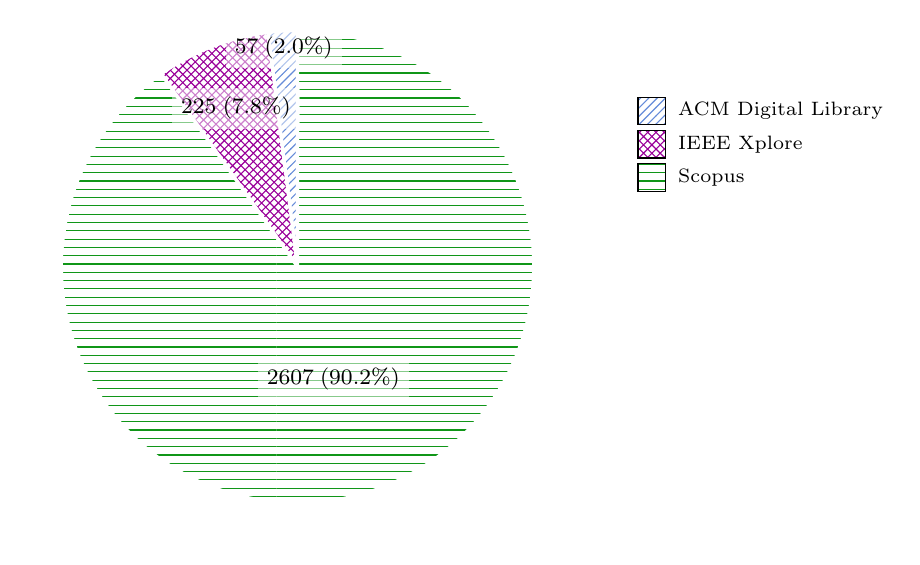
\begin{tikzpicture}
[
    pie chart,
    slice type={acm}{blu}{north east lines},
    slice type={ieee}{viola}{crosshatch},
    slice type={scopus}{verde}{horizontal lines},
    pie values/.style={font={\footnotesize}, fill=gray!0},
    scale=3
]
    \centering
    \pie{}{
        2.0/acm/57,
        7.8/ieee/225,
        90.2/scopus/2607}

    \legendchart[shift={(1.5cm,0.8cm)}]{
        {ACM Digital Library}/acm,
        {IEEE Xplore}/ieee,
        {Scopus}/scopus}
\end{tikzpicture}

    \caption{Estudos por Base de Dados.}
    \label{fig:papers-per-db}
\end{figure}

\subsubsection{Seleção dos Estudos}\label{sec:study-selection}
Na primeira fase da seleção, foram identificados e removidos 216 artigos duplicados. Em seguida, os critérios de inclusão e exclusão foram aplicados através da análise de títulos e resumos. Como resultado dessa triagem, 312 estudos foram considerados potencialmente relevantes e selecionados para leitura completa na fase seguinte.

\subsubsection{Avaliação de Qualidade dos Estudos}\label{sec:quality-evaluation}
Dos 312 estudos potencialmente relevantes, 138 foram submetidos à leitura completa e avaliação de qualidade com base nas Questões de Qualidade (QQ) definidas na Seção~\ref{sec:study-quality-criteria}. Após essa análise rigorosa, 67 estudos foram classificados como ``Excelente'' e aceitos para inclusão na síntese final, atendendo plenamente aos critérios de qualidade estabelecidos e apresentando contribuições relevantes para responder às questões de pesquisa.

A Figura~\ref{fig:quality-papers-evaluation} apresenta a distribuição dos 138 estudos de acordo com a classificação obtida na avaliação de qualidade. Dos estudos avaliados, 67 (48,6\%) foram classificados como ``Excelente'', 24 (17,4\%) como ``Muito Bom'', 3 (2,2\%) como ``Bom'', 4 (2,9\%) como ``Regular'', 1 (0,7\%) como ``Ruim'' e 39 (28,3\%) como ``Péssimo''.

\begin{figure}[!htb]
    \centering
    % ===========================================================================================
% Quality Classification of Studies - Pie Chart
% Study classification in quality assessment
% Total: 138 studies evaluated
% ===========================================================================================
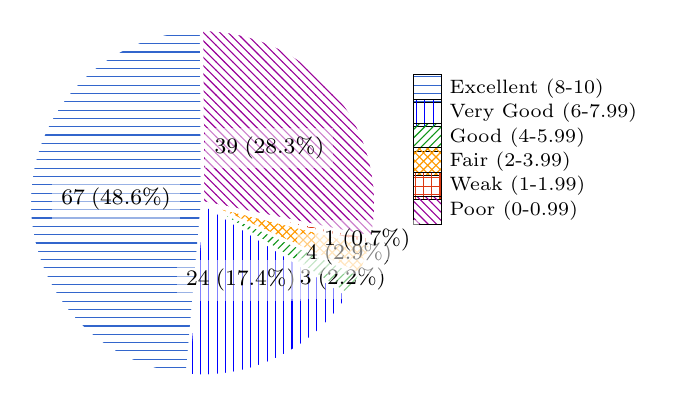
\begin{tikzpicture}
[
    pie chart,
    slice type={excelente}{hardblue}{horizontal lines},
    slice type={muitobom}{blue}{vertical lines},
    slice type={bom}{verde}{north east lines},
    slice type={regular}{giallo}{crosshatch},
    slice type={ruim}{rosso}{grid},
    slice type={pessimo}{viola}{north west lines},
    pie values/.style={font={\small}, fill=gray!0},
    scale=2.2
]
    \pie{}{
        48.6/excelente/67,
        17.4/muitobom/24,
        2.2/bom/3,
        2.9/regular/4,
        0.7/ruim/1,
        28.3/pessimo/39}

    \legendchart[shift={(1.3cm,0.8cm)}]{
        {Excellent (8-10)}/excelente,
        {Very Good (6-7.99)}/muitobom,
        {Good (4-5.99)}/bom,
        {Fair (2-3.99)}/regular,
        {Weak (1-1.99)}/ruim,
        {Poor (0-0.99)}/pessimo}
\end{tikzpicture}

    \caption{Classificação dos Estudos na Avaliação de Qualidade.}
    \label{fig:quality-papers-evaluation}
\end{figure}

\subsubsection{Extração de Dados}\label{sec:data-extraction}
A extração de dados foi realizada nos 67 estudos incluídos, utilizando um formulário estruturado com 33 questões de extração (QE), organizadas em questões fechadas (12 questões com categorias predefinidas) e questões abertas (21 questões para captura de informações qualitativas). A taxa de resposta variou conforme a natureza da questão: questões sobre identificação do modelo, contexto de aplicação e fatores de sucesso obtiveram taxas próximas a 100\%, enquanto questões mais específicas sobre licenciamento e periodicidade de cobrança apresentaram taxas menores (37-39\%), indicando que nem todos os estudos abordam esses aspectos operacionais.

Para a análise qualitativa das questões abertas, foi desenvolvido um esquema de codificação com 61 códigos organizados em 9 classes e 35 subclasses, resultando em 4.630 classificações de \textit{quotes} extraídas dos estudos. Esse processo de codificação permitiu identificar padrões, categorizar conceitos recorrentes e estabelecer relações entre os diferentes aspectos dos modelos de negócios analisados.





\section{Análise dos Resultados}\label{sec:analysis}

This section presents the results of the analysis of the 67 studies included in the systematic review, organized according to the research questions defined in Section~\ref{sec:research-questions}.

\subsection{RQ1: Business Model Identification and Taxonomy}

A análise dos estudos permitiu identificar um conjunto diversificado de modelos de negócios aplicados à indústria de software. A Tabela~\ref{tab:business-models-distribution} apresenta os principais modelos identificados e sua frequência nos estudos analisados.

\begin{table}[!htb]
\renewcommand{\arraystretch}{1.3}
\caption{Distribuição dos Principais Modelos de Negócios Identificados}
\label{tab:business-models-distribution}
\centering
\small
\begin{tabular}{lrr}
\toprule
\textbf{Modelo de Negócio} & \textbf{Menções} & \textbf{\%} \\
\midrule
\rowcolor{gray!15} Platform business model & 391 & 8,4\% \\
SaaS (Software as a Service) & 289 & 6,2\% \\
\rowcolor{gray!15} Mobile app market & 279 & 6,0\% \\
Freemium model & 264 & 5,7\% \\
\rowcolor{gray!15} Open source business model & 188 & 4,1\% \\
B2B business model & 161 & 3,5\% \\
\rowcolor{gray!15} Subscription-based pricing & 153 & 3,3\% \\
Cloud delivery model & 152 & 3,3\% \\
\rowcolor{gray!15} Service-oriented model & 144 & 3,1\% \\
Network effects & 133 & 2,9\% \\
\midrule
\textbf{Total de classificações} & \textbf{4.630} & \textbf{100\%} \\
\bottomrule
\end{tabular}
\vspace{0.2cm}

\footnotesize\textit{Nota: Percentuais calculados sobre o total de 4.630 classificações de quotes. Um mesmo estudo pode mencionar múltiplos modelos.}
\end{table}


O modelo de \textit{Platform business model} foi o mais frequentemente discutido, aparecendo em 391 menções nos estudos, seguido pelo \textit{Software as a Service} (SaaS) com 289 menções. O mercado de aplicativos móveis (\textit{Mobile app market}) representou 279 menções, evidenciando a relevância deste segmento. O modelo \textit{Freemium} apareceu em 264 menções, demonstrando sua popularidade como estratégia de monetização. Modelos baseados em \textit{Open source} foram identificados em 188 menções.

Em relação ao modo de entrega, 71,6\% dos estudos mencionaram o modelo \textit{Multi-tenant SaaS} como forma predominante de disponibilização de software. O modelo de entrega em nuvem (\textit{Cloud delivery}) foi referenciado em 152 menções, confirmando a tendência de migração para infraestruturas baseadas em cloud.

Quanto às fontes de receita, o modelo de \textit{Subscription} (assinatura) foi identificado como principal fonte em 76,1\% dos estudos, seguido por \textit{Usage/consumption} (consumo baseado em uso) com 41,8\% e \textit{Transaction} (transacional) com 32,8\%. Modelos baseados em publicidade (\textit{Advertising}) representaram 19,4\% dos estudos, particularmente relevantes em aplicativos móveis e plataformas freemium. A Figura~\ref{fig:revenue-sources} ilustra a distribuição das fontes de receita identificadas.

\begin{figure}[!htb]
    \centering
    % ===========================================================================================
% Revenue Sources - Horizontal Bar Chart
% Revenue sources identified in the studies
% Total: 67 studies
% ===========================================================================================
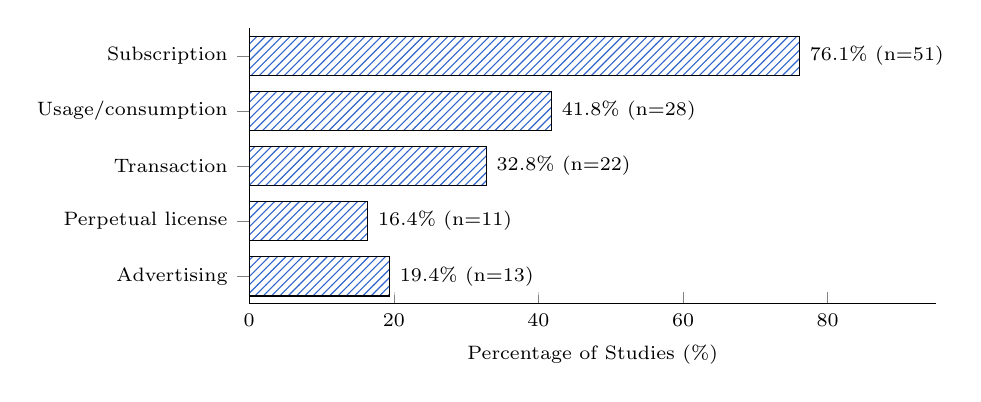
\begin{tikzpicture}
\begin{axis}[
    xbar,
    bar width=6pt,
    legend cell align=left,
    legend style={
        legend columns=1,
        at={(1.02,0.5)},
        anchor=west,
        draw=none,
        font=\scriptsize
    },
    ytick=data,
    axis y line*=none,
    axis x line*=bottom,
    x tick label style={font=\scriptsize},
    y tick label style={font=\scriptsize},
    label style={font=\scriptsize},
    xlabel={Percentage of Studies (\%)},
    xtick={0,20,40,60,80},
    xmin=0,
    xmax=95,
    width=0.85\columnwidth,
    height=4.5cm,
    bar width=5mm,
    yticklabels={
        {Advertising},
        {Perpetual license},
        {Transaction},
        {Usage/consumption},
        {Subscription}
    },
    area legend,
    y=7mm,
    enlarge y limits={abs=0.5},
    nodes near coords,
    nodes near coords align=horizontal,
    every node near coord/.append style={
        black,
        font=\scriptsize,
        text opacity=1,
        fill=white,
        fill opacity=0.6,
        outer sep=\pgflinewidth
    },
    visualization depends on={\thisrow{n} \as \mycount},
    nodes near coords={\pgfmathprintnumber\pgfplotspointmeta\% (n=\pgfmathprintnumber[fixed,precision=0]{\mycount})}
]
\addplot[pattern color=hardblue, pattern=north east lines] table [x=perc, y=idx, meta=perc] {
perc idx n
19.4 1 13
16.4 2 11
32.8 3 22
41.8 4 28
76.1 5 51
};
\end{axis}
\end{tikzpicture}

    \caption{Fontes de Receita Identificadas nos Estudos.}
    \label{fig:revenue-sources}
\end{figure}

\subsection{RQ2: Application Context and Market Segmentation}

Os fatores que influenciam a escolha do modelo de monetização podem ser categorizados em: tipo de cliente, tipo de produto/serviço, canais de aquisição e efeitos de rede.

\subsubsection{Tipo de Cliente-Alvo}

A análise revelou que 53,7\% dos estudos focaram em modelos \textit{Business-to-Business} (B2B), enquanto 41,8\% abordaram modelos \textit{Business-to-Consumer} (B2C). O segmento \textit{Enterprise} foi detalhado em 7,5\% dos estudos, enquanto o foco em pequenas e médias empresas (SME) apareceu em 35,8\%. Notavelmente, muitos estudos abordaram múltiplos segmentos simultaneamente, indicando a flexibilidade dos modelos de negócios de software em atender diferentes públicos. A Figura~\ref{fig:customer-types} apresenta a distribuição dos tipos de cliente-alvo.

\begin{figure}[!htb]
    \centering
    % ===========================================================================================
% Customer Types - Horizontal Bar Chart
% Target customer types identified in the studies
% Total: 67 studies
% ===========================================================================================
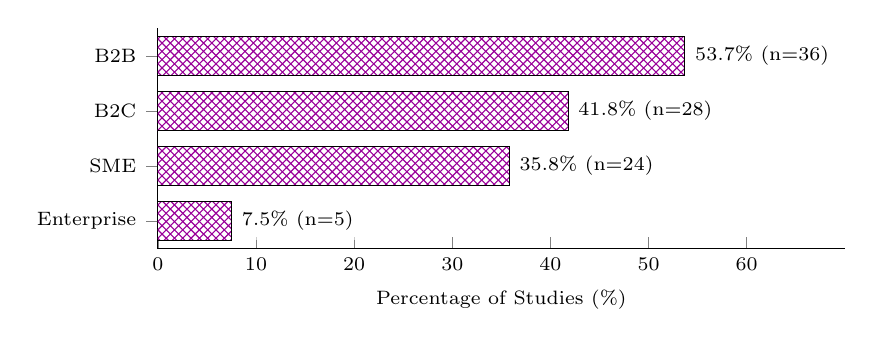
\begin{tikzpicture}
\begin{axis}[
    xbar,
    bar width=6pt,
    legend cell align=left,
    legend style={
        legend columns=1,
        at={(1.02,0.5)},
        anchor=west,
        draw=none,
        font=\scriptsize
    },
    ytick=data,
    axis y line*=none,
    axis x line*=bottom,
    x tick label style={font=\scriptsize},
    y tick label style={font=\scriptsize},
    label style={font=\scriptsize},
    xlabel={Percentage of Studies (\%)},
    xtick={0,10,20,30,40,50,60},
    xmin=0,
    xmax=70,
    width=0.85\columnwidth,
    height=4.5cm,
    bar width=5mm,
    yticklabels={
        {Enterprise},
        {SME},
        {B2C},
        {B2B}
    },
    area legend,
    y=7mm,
    enlarge y limits={abs=0.5},
    nodes near coords,
    nodes near coords align=horizontal,
    every node near coord/.append style={
        black,
        font=\scriptsize,
        text opacity=1,
        fill=white,
        fill opacity=0.6,
        outer sep=\pgflinewidth
    },
    visualization depends on={\thisrow{n} \as \mycount},
    nodes near coords={\pgfmathprintnumber\pgfplotspointmeta\% (n=\pgfmathprintnumber[fixed,precision=0]{\mycount})}
]
\addplot[pattern color=viola, pattern=crosshatch] table [x=perc, y=idx, meta=perc] {
perc idx n
7.5 1 5
35.8 2 24
41.8 3 28
53.7 4 36
};
\end{axis}
\end{tikzpicture}

    \caption{Tipos de Cliente-Alvo Identificados.}
    \label{fig:customer-types}
\end{figure}

\subsubsection{Tipo de Produto ou Serviço}

Quanto ao tipo de oferta, 89,6\% dos estudos trataram de \textit{Applications} (aplicações de software), e 79,1\% abordaram \textit{Platforms} (plataformas). Serviços gerenciados (\textit{Managed Services}) foram discutidos em 35,8\% dos estudos, enquanto \textit{Infrastructure} (infraestrutura) representou 13,4\%. APIs foram mencionadas em 7,5\% dos estudos como forma de entrega de valor.

\subsubsection{Canais de Aquisição de Clientes}

Os canais de aquisição mais frequentes foram: \textit{Direct sales} (vendas diretas) em 47,8\% dos estudos, \textit{Product-led Growth} (crescimento liderado pelo produto) em 41,8\%, \textit{Partners/channels} (parceiros e canais) em 38,8\%, e \textit{Digital marketing} em 37,3\%. O uso de \textit{Marketplaces} como canal de distribuição foi identificado em 22,4\% dos estudos. A Figura~\ref{fig:customer-channels} apresenta a distribuição dos canais de aquisição.

\begin{figure}[!htb]
    \centering
    % ===========================================================================================
% Customer Acquisition Channels - Horizontal Bar Chart
% Customer acquisition channels identified in the studies
% Total: 67 studies
% ===========================================================================================
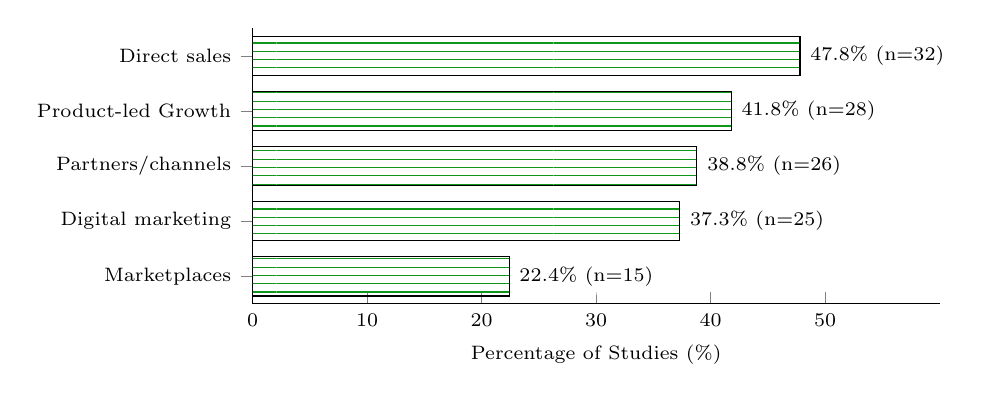
\begin{tikzpicture}
\begin{axis}[
    xbar,
    bar width=6pt,
    legend cell align=left,
    legend style={
        legend columns=1,
        at={(1.02,0.5)},
        anchor=west,
        draw=none,
        font=\scriptsize
    },
    ytick=data,
    axis y line*=none,
    axis x line*=bottom,
    x tick label style={font=\scriptsize},
    y tick label style={font=\scriptsize},
    label style={font=\scriptsize},
    xlabel={Percentage of Studies (\%)},
    xtick={0,10,20,30,40,50},
    xmin=0,
    xmax=60,
    width=0.85\columnwidth,
    height=5cm,
    bar width=5mm,
    yticklabels={
        {Marketplaces},
        {Digital marketing},
        {Partners/channels},
        {Product-led Growth},
        {Direct sales}
    },
    area legend,
    y=7mm,
    enlarge y limits={abs=0.5},
    nodes near coords,
    nodes near coords align=horizontal,
    every node near coord/.append style={
        black,
        font=\scriptsize,
        text opacity=1,
        fill=white,
        fill opacity=0.6,
        outer sep=\pgflinewidth
    },
    visualization depends on={\thisrow{n} \as \mycount},
    nodes near coords={\pgfmathprintnumber\pgfplotspointmeta\% (n=\pgfmathprintnumber[fixed,precision=0]{\mycount})}
]
\addplot[pattern color=verde, pattern=horizontal lines] table [x=perc, y=idx, meta=perc] {
perc idx n
22.4 1 15
37.3 2 25
38.8 3 26
41.8 4 28
47.8 5 32
};
\end{axis}
\end{tikzpicture}

    \caption{Canais de Aquisição de Clientes.}
    \label{fig:customer-channels}
\end{figure}

\subsubsection{Efeitos de Rede}

Os efeitos de rede foram categorizados em três tipos principais: efeitos diretos (\textit{Direct network effects} --- mais usuários geram mais valor) em 35,8\% dos estudos; efeitos cruzados (\textit{Cross-sided effects} --- grupos distintos se beneficiam mutuamente) em 31,3\%; e efeitos baseados em dados (\textit{Data network effects} --- mais dados melhoram o produto) em 22,4\%. A presença de efeitos de rede foi identificada como fator determinante na escolha de modelos de plataforma e marketplace. A Figura~\ref{fig:network-effects} ilustra a distribuição dos tipos de efeitos de rede.

\begin{figure}[!htb]
    \centering
    % ===========================================================================================
% Network Effects Types - Pie Chart
% Tipos de Efeitos de Rede identificados
% ===========================================================================================
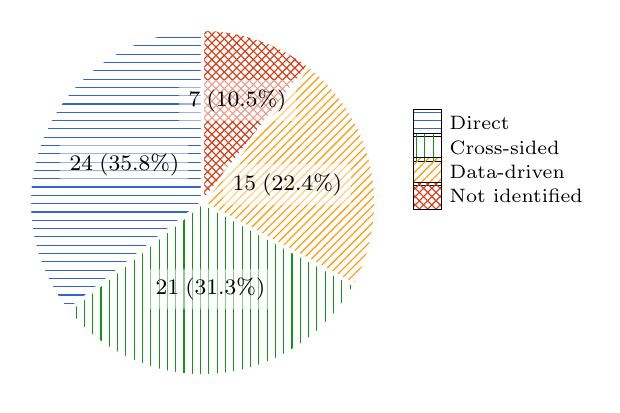
\begin{tikzpicture}
[
    pie chart,
    slice type={direct}{hardblue}{horizontal lines},
    slice type={cross}{verde}{vertical lines},
    slice type={data}{giallo}{north east lines},
    slice type={none}{rosso}{crosshatch},
    pie values/.style={font={\small}, fill=gray!0},
    scale=2.2
]
    \pie{}{
        35.8/direct/24,
        31.3/cross/21,
        22.4/data/15,
        10.5/none/7}

    \legendchart[shift={(1.3cm,0.6cm)}]{
        {Direct}/direct,
        {Cross-sided}/cross,
        {Data-driven}/data,
        {Not identified}/none}
\end{tikzpicture}

    \caption{Tipos de Efeitos de Rede Identificados.}
    \label{fig:network-effects}
\end{figure}

\subsection{RQ8: Temporal Evolution and Future Trends}

A análise temporal e temática dos estudos revelou tendências emergentes nos modelos de negócios de software. O código \textit{Technology evolution} (evolução tecnológica) foi identificado em 83 menções, indicando a importância da adaptação tecnológica contínua. O potencial de crescimento futuro (\textit{Future growth potential}) apareceu em 49 menções.

Em termos de maturidade dos modelos, 85 menções foram classificadas como modelos em crescimento (\textit{Growing business model}), 80 como modelos emergentes (\textit{Emerging business model}) e 23 como modelos consolidados (\textit{Consolidated business model}).

Quanto ao uso de marketplaces e plataformas de distribuição, a \textit{Apple App Store} foi mencionada em 20,9\% dos estudos e a \textit{Google Play Store} em 19,4\%, evidenciando a dominância das lojas de aplicativos móveis. Os marketplaces de nuvem empresarial (AWS, Azure, Google Cloud) ainda apresentaram baixa penetração nos estudos (3\% cada), sugerindo uma área em crescimento.

Tendências específicas identificadas incluem: a integração de sustentabilidade ecológica nos modelos de negócios digitais; a convergência entre transformação digital e sustentável; o crescimento de modelos baseados em \textit{Everything as a Service} (XaaS); e a importância crescente de dados e inteligência artificial na criação de valor.

\subsection{RQ6 \& RQ7: Success Factors, Challenges, and Mitigation Practices}

\subsubsection{Fatores de Sucesso}

Os principais fatores de sucesso identificados foram organizados em cinco categorias:

\begin{enumerate}
    \item \textbf{Gestão do ecossistema} (\textit{Ecosystem management}): Com 138 menções, foi o fator mais citado. Envolve o gerenciamento eficaz de relacionamentos com parceiros, desenvolvedores e stakeholders.

    \item \textbf{Expansão de mercado} (\textit{Market expansion}): Identificado em 84 menções, refere-se à estratégia de ampliação da base de clientes para alcançar economias de escala.

    \item \textbf{Preparação organizacional} (\textit{Organizational preparedness}): Com 64 menções, destaca a importância da prontidão da empresa para implementar mudanças no modelo de negócios.

    \item \textbf{Melhoria da qualidade do serviço} (\textit{Service quality improvement}): Presente em 36 menções, enfatiza a necessidade de aprimoramento contínuo para retenção de clientes.

    \item \textbf{Orientação baseada em valor} (\textit{Value-based orientation}): Com 36 menções, representa a estratégia de foco na entrega de valor percebido pelo cliente.
\end{enumerate}

A Figura~\ref{fig:success-factors} apresenta a distribuição dos fatores de sucesso identificados.

\begin{figure}[!htb]
    \centering
    % ===========================================================================================
% Success Factors - Horizontal Bar Chart
% Fatores de Sucesso identificados na literatura
% ===========================================================================================
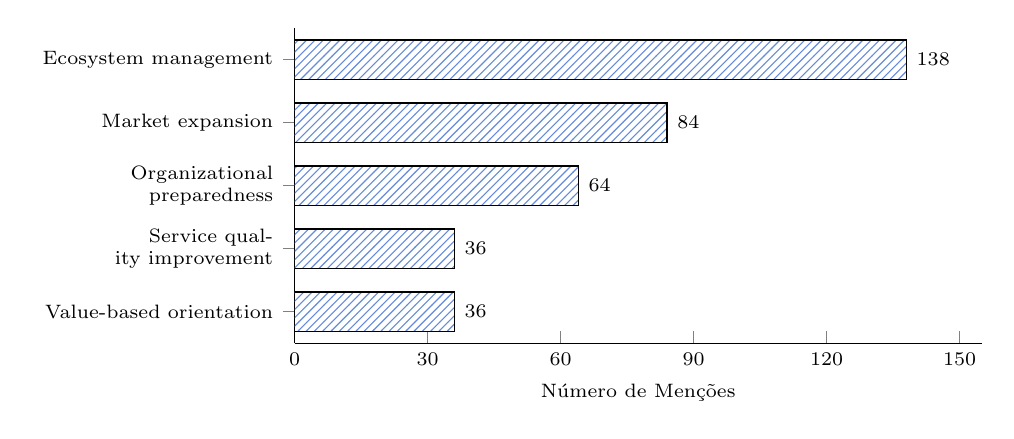
\begin{tikzpicture}
\begin{axis}[
    xbar,
    bar width=6pt,
    legend cell align=left,
    legend style={
        legend columns=1,
        at={(1.02,0.5)},
        anchor=west,
        draw=none,
        font=\scriptsize
    },
    ytick=data,
    axis y line*=none,
    axis x line*=bottom,
    x tick label style={font=\scriptsize},
    y tick label style={font=\scriptsize, text width=3cm, align=right},
    label style={font=\scriptsize},
    xlabel={Número de Menções},
    xtick={0,30,60,90,120,150},
    xmin=0,
    xmax=155,
    width=0.85\columnwidth,
    height=5cm,
    bar width=5mm,
    yticklabels={
        {Value-based orientation},
        {Service quality improvement},
        {Organizational preparedness},
        {Market expansion},
        {Ecosystem management}
    },
    area legend,
    y=8mm,
    enlarge y limits={abs=0.5},
    nodes near coords,
    nodes near coords align=horizontal,
    every node near coord/.append style={
        black,
        font=\scriptsize,
        text opacity=1,
        fill=white,
        fill opacity=0.6,
        outer sep=\pgflinewidth
    }
]
\addplot[pattern color=blu, pattern=north east lines] coordinates
{(36,1)(36,2)(64,3)(84,4)(138,5)};
\end{axis}
\end{tikzpicture}

    \caption{Fatores de Sucesso na Implementação de Modelos de Negócios.}
    \label{fig:success-factors}
\end{figure}

\subsubsection{Desafios de Implementação}

Os principais desafios identificados foram categorizados conforme a Tabela~\ref{tab:implementation-challenges}:

\begin{table}[!htb]
\renewcommand{\arraystretch}{1.3}
\caption{Identified Implementation Challenges}
\label{tab:implementation-challenges}
\centering
\small
\begin{tabular}{p{4cm}p{2.5cm}r}
\toprule
\textbf{Challenge} & \textbf{Category} & \textbf{Mentions} \\
\midrule
\rowcolor{gray!15} Security concerns & Customer barriers & 41 \\
Revenue stream transformation & Financial impact & 38 \\
\rowcolor{gray!15} Organizational readiness & Customer barriers & 23 \\
Partner ecosystem disruption & Ecosystem impact & 23 \\
\rowcolor{gray!15} Customer trust maintenance & Customer barriers & 19 \\
Quality management & Operational impact & 15 \\
\midrule
\textbf{Total} & & \textbf{159} \\
\bottomrule
\end{tabular}
\vspace{0.2cm}

\footnotesize\textit{Note: Challenges identified through qualitative coding of open-ended questions.}
\end{table}


\begin{enumerate}
    \item \textbf{Preocupações com segurança} (\textit{Security concerns}): Com 41 menções, representa a principal barreira identificada pelos clientes, especialmente em modelos baseados em nuvem.

    \item \textbf{Transformação do fluxo de receita} (\textit{Revenue stream transformation}): Identificada em 38 menções, refere-se ao desafio de migrar de pagamentos únicos para modelos de receita recorrente.

    \item \textbf{Prontidão organizacional do cliente} (\textit{Organizational readiness}): Com 23 menções, destaca a capacidade das organizações clientes de adotar novos modelos de negócio.

    \item \textbf{Disrupção do ecossistema de parceiros} (\textit{Partner ecosystem disruption}): Presente em 23 menções, evidencia o impacto das mudanças de modelo de negócios nos relacionamentos com parceiros e revendedores.

    \item \textbf{Manutenção da confiança do cliente} (\textit{Customer trust maintenance}): Com 19 menções, representa o desafio de manter a confiança durante transições de modelo de negócio.
\end{enumerate}

\subsubsection{Mitigation Practices (RQ7 continued)}

As práticas identificadas para mitigar os desafios de implementação foram:

\begin{enumerate}
    \item \textbf{Estratégias de precificação flexíveis} (\textit{Flexible pricing strategies}): Com 58 menções, foi a prática mais citada. Envolve a adaptação de modelos de precificação para acomodar diferentes necessidades e perfis de clientes.

    \item \textbf{Adoção de modelo híbrido} (\textit{Hybrid model adoption}): Identificada em 13 menções, refere-se à estratégia de manter simultaneamente modelos antigos e novos durante períodos de transição.

    \item \textbf{Implementação piloto} (\textit{Pilot implementation}): Com 8 menções, representa a abordagem de realizar implantações controladas com clientes selecionados antes da adoção em larga escala.

    \item \textbf{Compensação de parceiros} (\textit{Partner compensation}): Presente em 3 menções, envolve suporte financeiro aos parceiros afetados por mudanças no modelo de negócios.
\end{enumerate}

\subsection{RQ3, RQ4, RQ5 \& RQ9: Business Model Characteristics}

As características dos modelos de negócios foram organizadas em dimensões conforme o esquema de codificação desenvolvido. A classe \textit{Business model characteristics} concentrou 2.290 quotes classificadas, representando a maior densidade de informações extraídas.

\subsubsection{Estratégias de Precificação}

Quatro estratégias principais foram identificadas:
\begin{itemize}
    \item \textbf{Subscription-based pricing} (153 menções): Modelo de pagamento recorrente com cobrança mensal ou anual pelo acesso ao software.
    \item \textbf{Pay-as-you-go pricing} (40 menções): Modelo baseado em consumo, onde o cliente paga pelo que utiliza.
    \item \textbf{Value-based pricing} (33 menções): Precificação baseada no valor percebido pelo cliente.
    \item \textbf{Cost-based pricing} (15 menções): Precificação baseada nos custos do fornecedor.
\end{itemize}

\subsubsection{Modelos de Receita}

Os principais modelos de receita identificados foram:
\begin{itemize}
    \item \textbf{Freemium model} (264 menções): Oferece versão básica gratuita com recursos premium pagos.
    \item \textbf{Open source business model} (188 menções): Baseado em software de código aberto com diversas estratégias de comercialização.
    \item \textbf{Data-driven monetization} (108 menções): Geração de receita a partir de dados e analytics.
    \item \textbf{Perpetual licensing} (14 menções): Modelo tradicional de licenciamento com pagamento único.
\end{itemize}

\subsubsection{Arquitetura Técnica}

A infraestrutura técnica foi caracterizada por:
\begin{itemize}
    \item \textbf{Cloud computing infrastructure} (95 menções): Infraestrutura habilitadora para entrega em nuvem.
    \item \textbf{Multi-tenant architecture} (24 menções): Arquitetura onde uma única instância serve múltiplos clientes.
    \item \textbf{On-demand access} (24 menções): Acesso ao software disponível imediatamente quando necessário.
    \item \textbf{Remote hosting} (18 menções): Software hospedado em servidores externos.
\end{itemize}

\subsubsection{Criação de Valor}

Os mecanismos de criação de valor incluem:
\begin{itemize}
    \item \textbf{Platform business model} (391 menções): Criação de valor através de ecossistemas de conexões externas.
    \item \textbf{Network effects} (133 menções): Benefício onde o valor aumenta com mais usuários.
    \item \textbf{Marketplace model} (63 menções): Facilitação de transações entre múltiplas partes.
\end{itemize}





\section{Discussão dos Resultados}\label{sec:discussion}

Esta seção discute as principais descobertas da revisão sistemática, apresentando uma síntese integrada dos resultados e suas implicações para pesquisadores e profissionais.

\subsection{Síntese dos Principais Achados}

A análise dos 67 estudos revelou um panorama rico e diversificado dos modelos de negócios de software. A predominância do modelo SaaS (76,1\% dos estudos mencionando \textit{subscription} como fonte de receita) confirma a transformação fundamental ocorrida na indústria de software na última década. Este modelo oferece vantagens tanto para fornecedores --- receita recorrente previsível, redução de pirataria, ciclos de atualização contínuos --- quanto para clientes --- menor investimento inicial, escalabilidade e acesso a atualizações constantes.

A forte presença de modelos de plataforma (391 menções) e os efeitos de rede associados (133 menções) evidenciam a importância crescente dos ecossistemas no mercado de software. Empresas bem-sucedidas não apenas vendem produtos, mas orquestram ecossistemas que conectam desenvolvedores, usuários e parceiros, criando valor através de efeitos de rede positivos.

O modelo \textit{freemium} (264 menções) emergiu como estratégia relevante, particularmente em mercados B2C e aplicativos móveis. Esta abordagem reduz barreiras de entrada para usuários, permitindo experimentação antes da conversão para versões pagas. Entretanto, os estudos indicam que o sucesso do \textit{freemium} depende de configurações específicas de fatores, não sendo universalmente aplicável.

\subsection{Padrões e Correlações Identificados}

A análise cruzada dos dados revelou padrões importantes:

\subsubsection{Correlação entre Tipo de Cliente e Canais de Aquisição}

Modelos B2B tendem a utilizar vendas diretas (75\%) e parceiros de canal (61\%), enquanto modelos B2C privilegiam \textit{Product-led Growth} (68\%), marketing digital (54\%) e marketplaces (39\%). Esta diferenciação reflete as distintas jornadas de compra e processos decisórios de cada segmento.

\subsubsection{Correlação entre Papel no Ecossistema e Efeitos de Rede}

Empresas com papel de plataforma bilateral (\textit{Two-sided platform}) apresentam predominantemente efeitos de rede cruzados (76\%), enquanto produtos \textit{standalone} mostram distribuição mais variada entre efeitos diretos (50\%) e ausência de efeitos de rede (30\%).

\subsubsection{Evolução dos Modelos de Precificação}

Os dados indicam uma evolução de modelos baseados em licenciamento perpétuo (14 menções) para modelos de assinatura (153 menções) e consumo (40 menções). Esta transição representa uma mudança fundamental na relação entre fornecedores e clientes, de transação única para relacionamento contínuo.

\subsection{Comparação com Literatura Prévia}

Os resultados desta revisão confirmam e expandem achados de estudos anteriores sobre modelos de negócios de software. A predominância do SaaS corrobora as previsões de crescimento identificadas em estudos do início da década. A importância dos efeitos de rede, destacada por \cite{keele2007guidelines}, foi confirmada empiricamente, com mais de um terço dos estudos identificando algum tipo de efeito de rede.

A identificação de desafios relacionados à transformação do fluxo de receita e à disrupção do ecossistema de parceiros adiciona detalhamento à literatura existente sobre transições de modelo de negócio. A literatura prévia frequentemente focava nos benefícios da migração para SaaS, enquanto esta revisão equilibra a perspectiva ao documentar sistematicamente os desafios enfrentados.

\subsection{Taxonomia Emergente}

Com base na análise, propõe-se uma taxonomia de modelos de negócios de software organizada em três dimensões principais:

\begin{enumerate}
    \item \textbf{Dimensão de Entrega}: Como o software é disponibilizado (SaaS multi-tenant, single-tenant, on-premises, híbrido, mobile).

    \item \textbf{Dimensão de Monetização}: Como a receita é gerada (subscription, usage-based, freemium, perpetual license, advertising, transaction fees).

    \item \textbf{Dimensão de Ecossistema}: Qual o papel da empresa e os mecanismos de criação de valor (standalone product, two-sided platform, marketplace, plugin/complement).
\end{enumerate}

Esta taxonomia permite classificar e comparar modelos de negócios de software de forma sistemática, facilitando a análise de opções estratégicas para empresas do setor.

\subsection{Implicações para a Prática}

Para profissionais e gestores de empresas de software, os resultados sugerem:

\begin{enumerate}
    \item \textbf{Estratégia de transição gradual}: A adoção de modelos híbridos durante períodos de transição reduz riscos e permite ajustes baseados em feedback do mercado.

    \item \textbf{Investimento em ecossistema}: O gerenciamento eficaz de parceiros e stakeholders é o fator de sucesso mais citado, indicando a necessidade de investimentos nessa área.

    \item \textbf{Flexibilidade de precificação}: Estratégias de precificação flexíveis que acomodem diferentes perfis de clientes são essenciais para maximizar adoção e receita.

    \item \textbf{Atenção à segurança}: Preocupações com segurança são a principal barreira identificada, exigindo investimentos em certificações, transparência e comunicação.

    \item \textbf{Alinhamento canal-cliente}: A escolha de canais de aquisição deve estar alinhada com o tipo de cliente-alvo (B2B vs. B2C).
\end{enumerate}

\subsection{Implicações para a Pesquisa}

Para pesquisadores, os achados indicam:

\begin{enumerate}
    \item \textbf{Lacuna em estudos experimentais}: Apenas 3\% dos estudos utilizaram métodos experimentais, indicando oportunidade para pesquisas que estabeleçam relações causais.

    \item \textbf{Subexploração de marketplaces cloud}: O baixo percentual de estudos sobre AWS Marketplace, Azure Marketplace e similares (3\% cada) sugere área emergente para investigação.

    \item \textbf{Necessidade de estudos longitudinais}: A maioria dos estudos apresenta visões transversais; estudos longitudinais sobre evolução de modelos de negócios são necessários.

    \item \textbf{Integração com sustentabilidade}: A emergência de modelos de negócios digitais sustentáveis representa fronteira de pesquisa promissora.
\end{enumerate}





\section{Ameaças à Validade do Estudo}\label{sec:threats}

Esta seção discute as principais ameaças à validade deste estudo, organizadas conforme as categorias propostas por \cite{petersen2008systematic}.

\subsection{Validade de Construto}

A validade de construto refere-se à adequação das medidas utilizadas para capturar os conceitos investigados.

\textbf{Definição das questões de pesquisa}: As questões de pesquisa foram definidas com base em revisões prévias da literatura e validadas através de discussões entre os pesquisadores. Entretanto, a amplitude das questões pode ter resultado em respostas heterogêneas, dificultando a síntese.

\textbf{Formulário de extração}: O formulário com 33 questões de extração foi desenvolvido iterativamente e testado em um subconjunto de estudos antes da aplicação completa. Apesar disso, algumas questões apresentaram taxas de resposta baixas (37-39\% para questões sobre licenciamento e periodicidade de cobrança), indicando possível desalinhamento entre as questões e o conteúdo dos estudos.

\textbf{Esquema de codificação}: Os 61 códigos utilizados na análise qualitativa foram desenvolvidos de forma iterativa através de processo indutivo-dedutivo. A validade da codificação foi verificada através de revisão cruzada de uma amostra de classificações.

\subsection{Validade Interna}

A validade interna refere-se à confiabilidade dos processos de condução do estudo.

\textbf{Viés de seleção}: A seleção de estudos foi realizada seguindo critérios predefinidos. Entretanto, a triagem de 2.889 artigos por um único pesquisador na fase inicial pode ter introduzido viés. Para mitigar esse risco, casos duvidosos foram discutidos com co-pesquisadores.

\textbf{Viés de extração}: A extração de dados foi realizada por um pesquisador, com verificação amostral por um segundo pesquisador. A taxa de concordância foi satisfatória, mas divergências pontuais podem ter ocorrido em casos ambíguos.

\textbf{Codificação qualitativa}: A atribuição de códigos às quotes extraídas envolveu julgamento interpretativo. Para aumentar a confiabilidade, foram desenvolvidas descrições detalhadas para cada código e realizadas revisões periódicas de consistência.

\subsection{Validade Externa}

A validade externa refere-se à generalização dos resultados.

\textbf{Escopo temporal}: O estudo limitou-se a publicações de 2014 a 2024, período que captura a maturação do modelo SaaS mas pode não refletir tendências mais recentes, como modelos baseados em inteligência artificial generativa.

\textbf{Escopo de bases de dados}: Foram utilizadas três bases de dados (ACM, IEEE Xplore, Scopus). Embora representativas da literatura em engenharia de software e sistemas de informação, estudos publicados em outras fontes (conferências de gestão, literatura cinzenta) podem não ter sido capturados.

\textbf{Viés de publicação}: Estudos publicados tendem a reportar resultados positivos ou significativos, potencialmente sub-representando experiências de fracasso ou resultados neutros na implementação de modelos de negócios.

\textbf{Contexto geográfico e industrial}: Os estudos analisados apresentam predominância de contextos norte-americanos e europeus, e de setores como aplicativos móveis e plataformas empresariais. A generalização para outros contextos deve ser feita com cautela.

\subsection{Confiabilidade}

A confiabilidade refere-se à possibilidade de replicação do estudo.

\textbf{Documentação do protocolo}: O protocolo de pesquisa foi documentado detalhadamente, incluindo string de busca, critérios de inclusão/exclusão e questões de extração. Os dados brutos e códigos de análise estão disponíveis em repositório público para verificação.

\textbf{Ferramentas utilizadas}: O uso combinado de ferramentas (Thoth e Google Sheets) para gerenciamento dos dados pode dificultar a replicação exata. Entretanto, os procedimentos foram documentados para permitir reprodução equivalente.

\subsection{Mitigações Adotadas}

Para mitigar as ameaças identificadas, foram adotadas as seguintes estratégias:

\begin{itemize}
    \item Definição prévia e documentação do protocolo de pesquisa;
    \item Desenvolvimento iterativo do formulário de extração com teste piloto;
    \item Criação de esquema de codificação hierárquico com definições explícitas;
    \item Revisão cruzada de amostras de seleção, extração e codificação;
    \item Disponibilização dos dados e materiais em repositório aberto;
    \item Triangulação de dados quantitativos (questões fechadas) e qualitativos (questões abertas).
\end{itemize}





\section{Conclusão}\label{sec:conclusion}

This study presented a systematic literature review on software business models, analyzing 67 studies published between 2014 and 2024. The research addressed the ten proposed research questions, contributing to the systematization of knowledge in the area.

\subsection{Principais Contribuições}

As principais contribuições deste trabalho são:

\begin{enumerate}
    \item \textbf{Mapeamento abrangente}: Identificação e categorização de 61 códigos organizados em 9 classes, representando diferentes aspectos dos modelos de negócios de software, desde características técnicas até fatores de sucesso e desafios.

    \item \textbf{Evidência quantitativa}: Consolidação de dados sobre a prevalência de diferentes modelos, com destaque para SaaS/subscription (76,1\%), plataformas (391 menções) e freemium (264 menções).

    \item \textbf{Taxonomia de modelos}: Proposição de uma taxonomia tridimensional (entrega, monetização, ecossistema) para classificação de modelos de negócios de software.

    \item \textbf{Síntese de desafios e mitigações}: Documentação sistemática de 159 menções a desafios de implementação e 82 menções a práticas de mitigação.

    \item \textbf{Identificação de tendências}: Mapeamento de tendências emergentes, incluindo a integração de sustentabilidade, efeitos de rede baseados em dados e modelos baseados em plataforma.
\end{enumerate}

\subsection{Answers to Research Questions}

\textbf{RQ1}: The most commonly used models are based on platforms, SaaS, freemium, and open source, with predominance of cloud delivery and subscription-based monetization.

\textbf{RQ2}: Models are implemented across diverse contexts, with 53.7\% focusing on B2B, 41.8\% on B2C, and varying distribution across vertical segments and company sizes.

\textbf{RQ3}: Technical characteristics include multi-tenant SaaS delivery (71.6\%), cloud infrastructure (95 mentions), multi-tenant architecture (24 mentions), and on-demand access (24 mentions).

\textbf{RQ4}: Monetization strategies include subscription (76.1\%), usage-based (41.8\%), and transaction-based (32.8\%), with pricing models varying from value-based to pay-as-you-go.

\textbf{RQ5}: Ecosystem dynamics involve platform roles (391 mentions), network effects (133 mentions), with go-to-market strategies including direct sales (47.8\%) and product-led growth (41.8\%).

\textbf{RQ6}: Main success factors are ecosystem management (138 mentions), market expansion (84), and organizational preparedness (64).

\textbf{RQ7}: Challenges include security concerns (41 mentions), revenue stream transformation (38), and partner disruption (23). Effective mitigation practices include flexible pricing strategies (58 mentions) and hybrid model adoption (13).

\textbf{RQ8}: Emerging trends include technology evolution (83 mentions), with 85 growing models and 80 emerging models identified.

\textbf{RQ9}: Models are characterized by delivery dimensions (SaaS multi-tenant, cloud), monetization dimensions (subscription, freemium), and ecosystem dimensions (platform, marketplace).

\textbf{RQ10}: Studies employ diverse methodologies, with predominance of case studies and empirical analyses, though experimental studies remain underrepresented (3\%).

\subsection{Trabalhos Futuros}

Com base nos resultados e lacunas identificadas, sugerem-se as seguintes direções para pesquisas futuras:

\begin{itemize}
    \item Desenvolvimento de uma ontologia formal para representação de modelos de negócios de software, permitindo raciocínio automatizado e suporte à decisão;

    \item Estudos experimentais que estabeleçam relações causais entre configurações de modelos de negócios e desempenho;

    \item Investigação aprofundada sobre modelos de negócios baseados em inteligência artificial e machine learning;

    \item Análise longitudinal da evolução de modelos de negócios em empresas específicas;

    \item Estudos sobre a eficácia de marketplaces cloud empresariais como canal de distribuição.
\end{itemize}

Os resultados consolidados desta revisão sistemática fornecem base conceitual sólida para o desenvolvimento de ferramentas e frameworks que apoiem pesquisadores e profissionais na compreensão, comparação e seleção de modelos de negócios para produtos de software.

% An example of a floating figure using the graphicx package.
% Note that \label must occur AFTER (or within) \caption.
% For figures, \caption should occur after the \includegraphics.
% Note that IEEEtran v1.7 and later has special internal code that
% is designed to preserve the operation of \label within \caption
% even when the captionsoff option is in effect. However, because
% of issues like this, it may be the safest practice to put all your
% \label just after \caption rather than within \caption{}.
%
% Reminder: the "draftcls" or "draftclsnofoot", not "draft", class
% option should be used if it is desired that the figures are to be
% displayed while in draft mode.
%
%\begin{figure}[!t]
%\centering
%\includegraphics[width=2.5in]{myfigure}
% where an .eps filename suffix will be assumed under latex,
% and a .pdf suffix will be assumed for pdflatex; or what has been declared
% via \DeclareGraphicsExtensions.
%\caption{Simulation results for the network.}
%\label{fig_sim}
%\end{figure}

% Note that the IEEE typically puts floats only at the top, even when this
% results in a large percentage of a column being occupied by floats.


% An example of a double column floating figure using two subfigures.
% (The subfig.sty package must be loaded for this to work.)
% The subfigure \label commands are set within each subfloat command,
% and the \label for the overall figure must come after \caption.
% \hfil is used as a separator to get equal spacing.
% Watch out that the combined width of all the subfigures on a
% line do not exceed the text width or a line break will occur.
%
%\begin{figure*}[!t]
%\centering
%\subfloat[Case I]{\includegraphics[width=2.5in]{box}%
%\label{fig_first_case}}
%\hfil
%\subfloat[Case II]{\includegraphics[width=2.5in]{box}%
%\label{fig_second_case}}
%\caption{Simulation results for the network.}
%\label{fig_sim}
%\end{figure*}
%
% Note that often IEEE papers with subfigures do not employ subfigure
% captions (using the optional argument to \subfloat[]), but instead will
% reference/describe all of them (a), (b), etc., within the main caption.
% Be aware that for subfig.sty to generate the (a), (b), etc., subfigure
% labels, the optional argument to \subfloat must be present. If a
% subcaption is not desired, just leave its contents blank,
% e.g., \subfloat[].


% An example of a floating table. Note that, for IEEE style tables, the
% \caption command should come BEFORE the table and, given that table
% captions serve much like titles, are usually capitalized except for words
% such as a, an, and, as, at, but, by, for, in, nor, of, on, or, the, to
% and up, which are usually not capitalized unless they are the first or
% last word of the caption. Table text will default to \footnotesize as
% the IEEE normally uses this smaller font for tables.
% The \label must come after \caption as always.
%
%\begin{table}[!t]
%% increase table row spacing, adjust to taste
%\renewcommand{\arraystretch}{1.3}
% if using array.sty, it might be a good idea to tweak the value of
% \extrarowheight as needed to properly center the text within the cells
%\caption{An Example of a Table}
%\label{table_example}
%\centering
%% Some packages, such as MDW tools, offer better commands for making tables
%% than the plain LaTeX2e tabular which is used here.
%\begin{tabular}{|c||c|}
%\hline
%One & Two\\
%\hline
%Three & Four\\
%\hline
%\end{tabular}
%\end{table}


% Note that the IEEE does not put floats in the very first column
% - or typically anywhere on the first page for that matter. Also,
% in-text middle ("here") positioning is typically not used, but it
% is allowed and encouraged for Computer Society conferences (but
% not Computer Society journals). Most IEEE journals/conferences use
% top floats exclusively.
% Note that, LaTeX2e, unlike IEEE journals/conferences, places
% footnotes above bottom floats. This can be corrected via the
% \fnbelowfloat command of the stfloats package.






% if have a single appendix:
%\appendix[Proof of the Zonklar Equations]
% or
%\appendix  % for no appendix heading
% do not use \section anymore after \appendix, only \section*
% is possibly needed

% use appendices with more than one appendix
% then use \section to start each appendix
% you must declare a \section before using any
% \subsection or using \label (\appendices by itself
% starts a section numbered zero.)
%


% \appendices
% \section{Proof of the First Zonklar Equation}
% Appendix one text goes here.

% % you can choose not to have a title for an appendix
% % if you want by leaving the argument blank
% \section{}
% Appendix two text goes here.


% use section* for acknowledgment
\section*{Acknowledgment}


The authors would like to thank...


% Can use something like this to put references on a page
% by themselves when using endfloat and the captionsoff option.
\ifCLASSOPTIONcaptionsoff
  \newpage
\fi



% trigger a \newpage just before the given reference
% number - used to balance the columns on the last page
% adjust value as needed - may need to be readjusted if
% the document is modified later
%\IEEEtriggeratref{8}
% The "triggered" command can be changed if desired:
%\IEEEtriggercmd{\enlargethispage{-5in}}

% references section

% can use a bibliography generated by BibTeX as a .bbl file
% BibTeX documentation can be easily obtained at:
% http://mirror.ctan.org/biblio/bibtex/contrib/doc/
% The IEEEtran BibTeX style support page is at:
% http://www.michaelshell.org/tex/ieeetran/bibtex/
\bibliographystyle{IEEEtran}

\bibliography{Referencias}
%
% <OR> manually copy in the resultant .bbl file
% set second argument of \begin to the number of references
% (used to reserve space for the reference number labels box)
% \begin{thebibliography}{1}

% \bibitem{IEEEhowto:kopka}
% H.~Kopka and P.~W. Daly, \emph{A Guide to \LaTeX}, 3rd~ed.\hskip 1em plus
%   0.5em minus 0.4em\relax Harlow, England: Addison-Wesley, 1999.

% \end{thebibliography}

% biography section
%
% If you have an EPS/PDF photo (graphicx package needed) extra braces are
% needed around the contents of the optional argument to biography to prevent
% the LaTeX parser from getting confused when it sees the complicated
% \includegraphics command within an optional argument. (You could create
% your own custom macro containing the \includegraphics command to make things
% simpler here.)
%\begin{IEEEbiography}[{\includegraphics[width=1in,height=1.25in,clip,keepaspectratio]{mshell}}]{Michael Shell}
% or if you just want to reserve a space for a photo:

\begin{IEEEbiography}{Michael Shell}
Biography text here.
\end{IEEEbiography}

% if you will not have a photo at all:
\begin{IEEEbiographynophoto}{John Doe}
Biography text here.
\end{IEEEbiographynophoto}

% insert where needed to balance the two columns on the last page with
% biographies
%\newpage

\begin{IEEEbiographynophoto}{Jane Doe}
Biography text here.
\end{IEEEbiographynophoto}

% You can push biographies down or up by placing
% a \vfill before or after them. The appropriate
% use of \vfill depends on what kind of text is
% on the last page and whether or not the columns
% are being equalized.

%\vfill

% Can be used to pull up biographies so that the bottom of the last one
% is flush with the other column.
%\enlargethispage{-5in}



% that's all folks
\end{document}
